\subsection{Outline}

Parameterization inputs include the litter box volume, maximum litter mass, and desired horizontal ($x$) and vertical ($y$) reach of the legs.
The litter mass is limited between $0\text{kg}$ and $5\text{kg}$, as per the project mandate. The litter box volume is limited between $5000\text{cm}^3$ and $15000\text{cm}^3$. These values were determined based on the project mandate and dimensions provided by group WR2B.
The maximum reach in $x$ and $y$ determine the obstacles the robot can navigate (for example: stairs, size of rocks, crevices). They are limited between $170\text{mm}$ and $405\text{mm}$, and $40\text{mm}$ and $95\text{mm}$ respectively. A different design solution would be required to operate outside these intervals, as detailed in the discussion.

Table \ref{tab:parametrized_parts} only lists the significant key components being parameterized based on the user inputs, as well as the range of their key parameterized dimensions. All components have parameterized dimensions which may not be shown in the table. 

\begin{table}
    \caption{Summary of parameterized parts (Str. : Structural, Geo. : Geometric)}
    \centering
    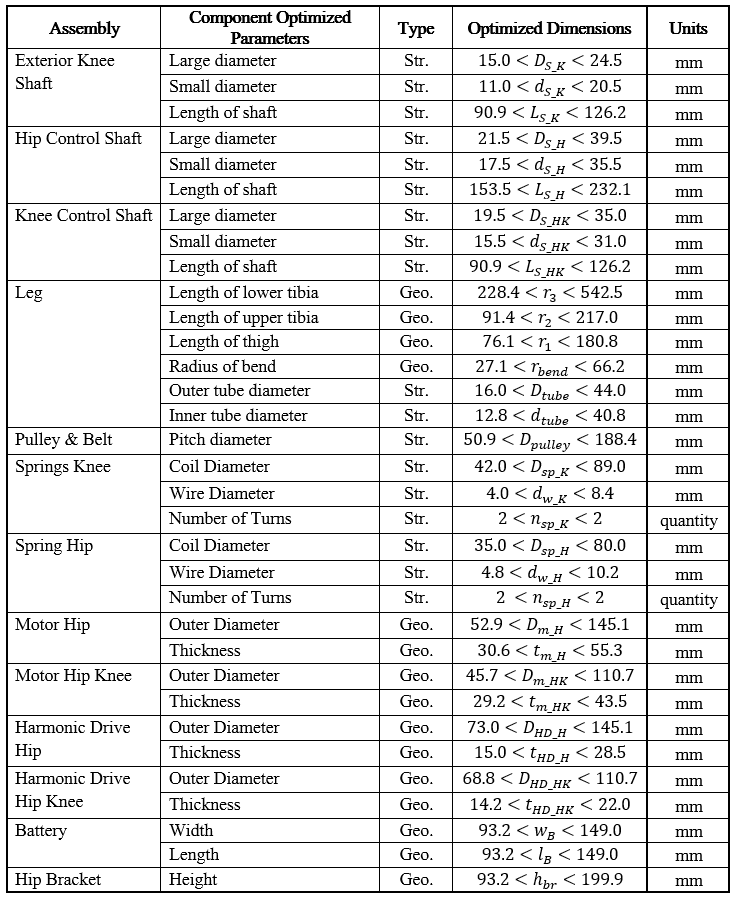
\includegraphics[width=\textwidth]{3_Parametrization/img/ParaTable.PNG}
    \label{tab:parametrized_parts}
\end{table}{}
